%!TEX root = thesis.tex

\chapter{Visualisation Refinement}
\label{chap:visualisation-refinement}

Following the first user study (see Chapter~\ref{chap:user-study}), limitations with both the visualisations and the evaluation method were identified and corrective steps were taken. The steps taken to correct these limitations and the resulting refined visualisation are outlined in this chapter.

\section{Rationale}

The intial user study (see Chapter~\ref{chap:user-study}) identified some improvement in enjoyment through the use of visualisations. However, the study had conflicting results regarding understanding with audiences reporting high levels of understanding attributed to the didactic visualisations when asked directly, but with lower overall understanding during the beginning stages of the live coding performance (see Section~\ref{section:user-study-understanding}). A new visualisation prototype was developed to bring together features identified as positively impacting enjoyment and understanding in one visualisation. This visualisation prototype built on a combination of the aesthetic and didactic visualisations evaluated in the previous study. The intention of this visualisation was to smooth the early transition into the more educational aspects of the visualisations through the aesthetic features identified.

Technical limitations identified in the previous iteration of the visualisation prototype including incorrect timing and beat, no direct feedback from the programmer and limited links between the visuals and the source code. 

The goal of this iteration of the visualisations was to align the mental model of the audience with that of the programmer, representing the state of the code visually and showing the iteraction of the programmer with the source code.

-stop the visualisation from obscuring the code, 

\section{Design}

As with the previous visualisation iteration, guidelines were identified, adapted and applied to the design process. A selection of the design guidelines are outlined below:

\begin{itemize}
\item Show relationships between entities using lines \cite[p.~183]{Ware2013a}~\glab{guide:links}
\item ``Consider using pictorial icons for pedagogical purposes in infographics.'' \cite[p.~320]{Ware2013a}~\glab{guide:icons}
\end{itemize}

Some more specific guidelines and improvement taken from the previous study included:

\begin{itemize}
\item ``\ldots relate every beat\ldots~to the code responsible for that beat'' (see Section~\ref{section:improvements})~\glab{guide:code-responsible}
\item Respond to the programmer's typing (see Section~\ref{section:liveness})~\glab{guide:typing}
\item Reduce visualisation distraction (see Section~\ref{section:user-study-discussion})~\glab{guide:distraction}

\end{itemize}


% \cite{Purchase1996}...

\begin{figure}
  \centering 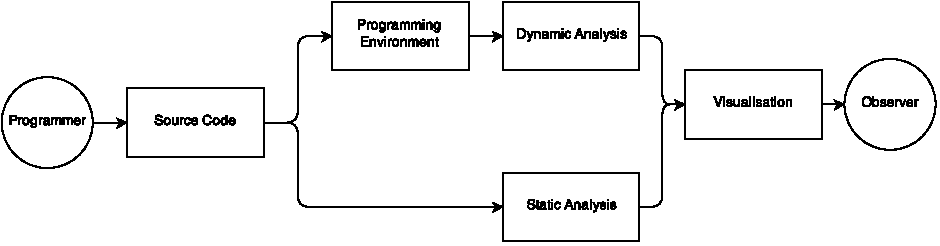
\includegraphics[width=\columnwidth]{../images/diagrams/knowledge-flow-refined.pdf}
  \caption{Knowledge flow from programmer to observer as directed by the visualisation technique employed.}
\label{fig:knowledge-flow-refined}
\end{figure}

Three sources of data were to be combined and visualised including the state of the source code, the state of the running program and the manipulation between the two by the live coder. To achieve this, three major components were required including an application manager, a code manager and an editor plugin (see Figure~\ref{fig:visualisation-class-diagram}). The following sections detail the implementation of these components.

This visualisation was, as with the previous iteration, rendered under the source code. 

% \cite{Heer2006} might be useful for explaining the design of this visualisation...

\begin{figure}
  \centering 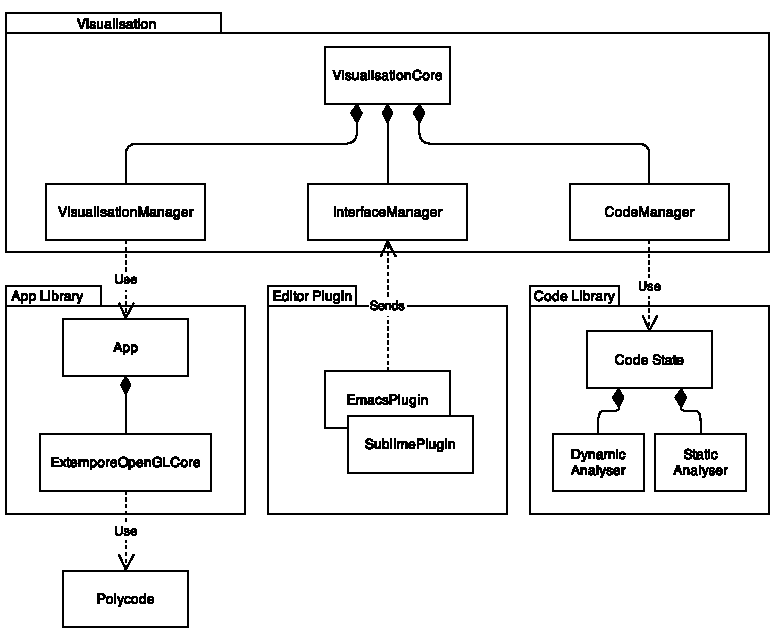
\includegraphics[width=\columnwidth]{../images/diagrams/visualisation-class-diagram.pdf}
  \caption[Prototype (second iteration) class diagram]{Class diagram of the visualisation technique employed. The three major components included the visualisation manager, the interface manager and the code manager.}
\label{fig:visualisation-class-diagram}
\end{figure}

\subsection{Visualisation Manager}

The visualisation manager handled all visual elements on the screen. The Polycode~\cite{Safrin2013} library was bound to the live coding environment allowing for more advanced two-dimensional graphical manipulations than the previous visualisation iteration through scene graph manipulation. Using this technique, the intention was to represent the state of the source code, the manipulation of the source code and the state of the active source code in the same visual environment.

\subsection{Interface Mananger}
\label{sec:interface-manager}

To gather information regarding the actions of the programmer, a method of interfacing with the live coder's programming environment (text editor) was required. This was acheived using a text editor plugin sending programmer actions over an \ac{OSC} protocol. The interactions sent included cursor movement, all source code changes, file focus and source code evaluation. This protocol was implemented as a standard way of communicating between the text editor in use and the visualisations. Table~\ref{table:osc-protocol} describes the protocol.

Two text editor plugins implementing the protocol were developed including a plugin for EMACS~\cite{Stallman1981} and a plugin for Sublime Text~\cite{Skinner2013}.

\begin{table}
  \centering
  \begin{tabular}{|l|p{4.75cm}|p{4.75cm}|}
  \hline
  \textbf{OSC Address} & \textbf{Arguments} & \textbf{Description}\\
  \hline
	/interface/code & source\_code & Sent when the source code within the text editor changes.\\
	\hline
	/interface/evaluate & evaluated\_code & Sent when a block of source code within the text editor is evaluated (activated). \\
	\hline
	/interface/error & error\_text & Sent when an error occurs within the text editor or the evaluation of source code fails.\\
	\hline
	/interface/focus & file\_name & Sent when the file currently being edited changes.\\
	\hline
	/interface/cursor & cursor\_position \newline screen\_minimum\_position \newline screen\_maximum\_position \newline cursor\_position\_x \newline cursor\_position\_y & Sent when the text editor cursor selection changes. \\
  \hline
  \end{tabular}
  \caption{The OSC protocol developed for standardised interaction between text editors and the visualisation.}
  \label{table:osc-protocol}
\end{table}

% /interface/selection"  data));; args: count start end start end... 
% /interface/code"  (event_get_data e)));; args: code
% /interface/evaluate"  (event_get_data e))) ;; args: evaluated_code
% /interface/keyboard"  data));; unused
% /interface/error"  (event_get_data e))) ;; args: message
% /interface/focus"  (event_get_data e))) ;; args: file_name
% /interface/cursor"  data))

\subsection{Code Manager}

Both static analysis of source code and the dynamic analysis (see~\cite{Eisenbarth2003} and~\cite{Jerding1997}) of the program were combined into this iteration of the visualisation prototype in order to provide the audience with a link between the \acf{SoW} and the \acf{SoC}~\cite{Swift2013}.
% {\color{red} explain what the \ac{SoW} and the \ac{SoC} actually is and show the link between the \ac{SoW} with dynamic analysis and the \ac{SoC} with static analysis...}

Static analysis of the source code involved parsing the source code written by the programmer and analysing any changes made, mapping these changes to historic source code states. The source code written by the programmer was sent from an editor plugin (see~\ref{sec:interface-manager}) to the Extempore visualisation program and stored as the current \ac{SoC}. Mappings to previous states were then made for each function within the source code.

Dynamic analysis of the running program involved providing mechanisms for the programmer to send running state information to be stored as the \ac{SoW}. A callback hook was provided to be used when creating an instrument during performance. This hook would provide data on the names of the instruments, the state of the callbacks and would allow links to be determined between the \ac{SoC} and the \ac{SoW}.

\subsection{Mappings}

\begin{figure}
\centering
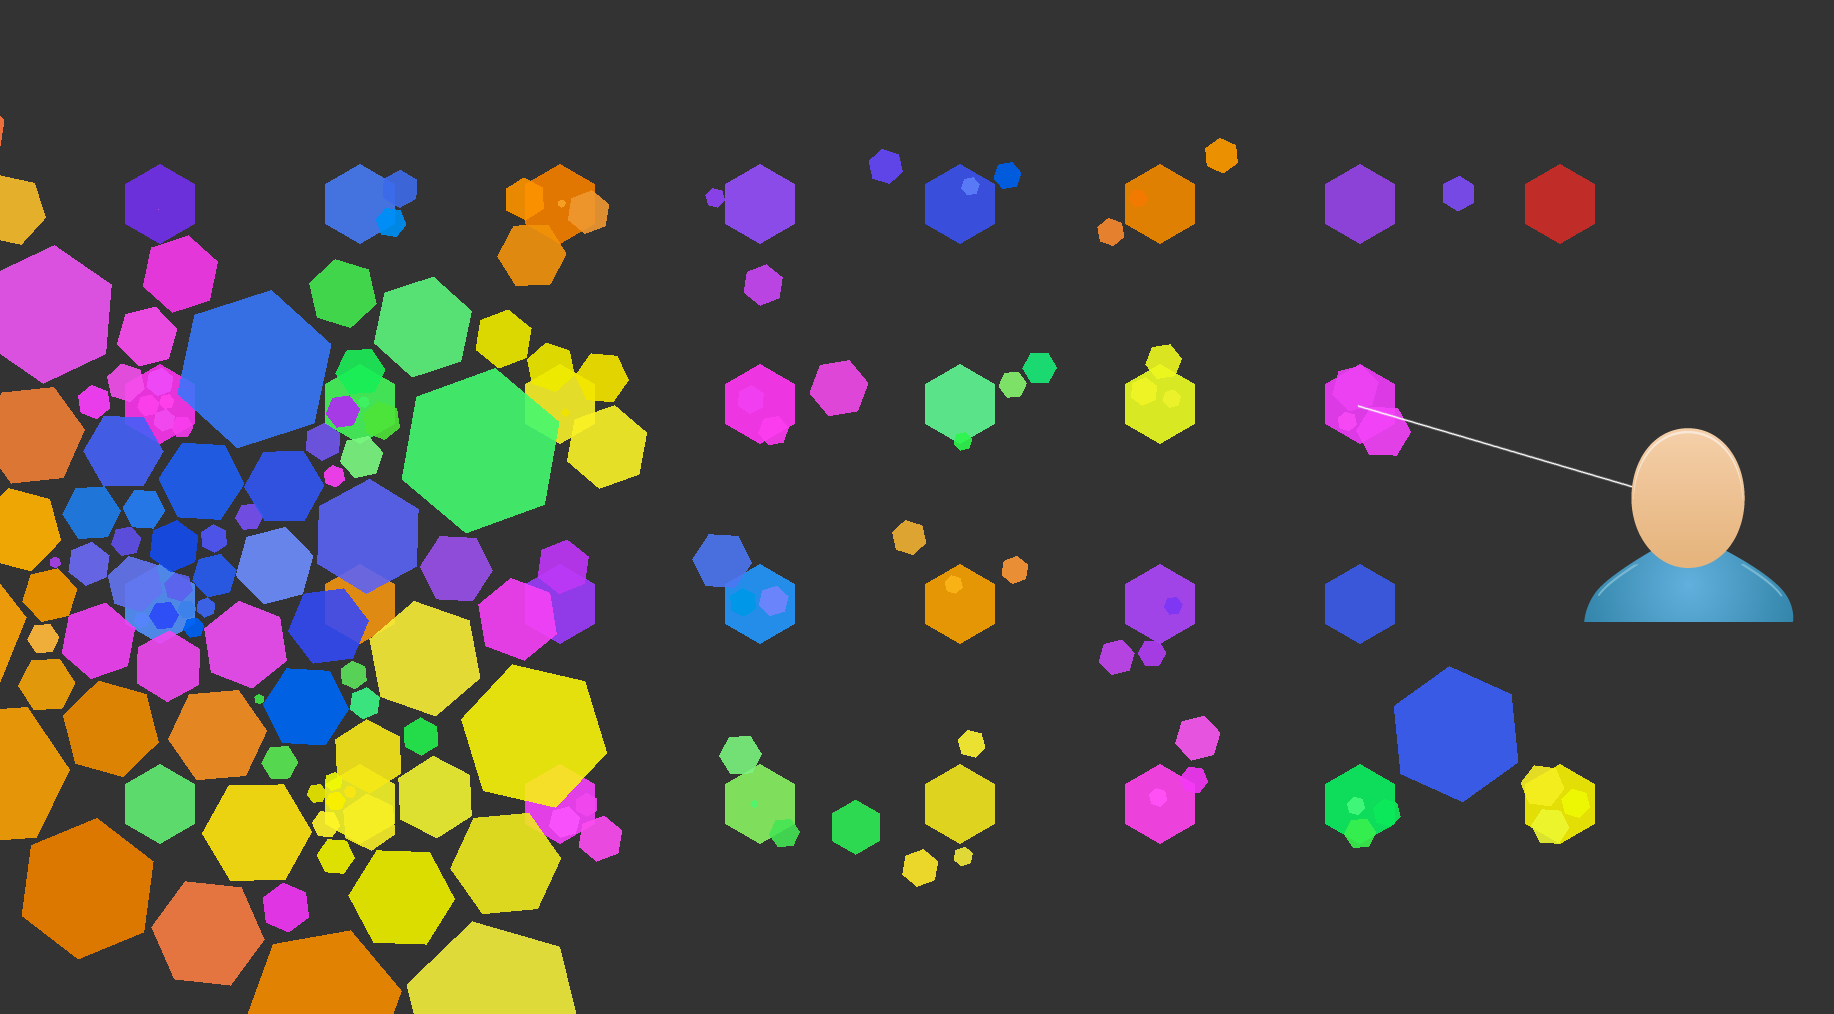
\includegraphics[width=\textwidth]{../images/final-visualisations/final-code-visualisation.png}
\caption[Prototype (second iteration) example]{An example of the visualisation developed.}
\label{fig:final-visualisation}
\end{figure}

A number of specific mappings were assigned to the visualisation. These visual mappings related directly to actions taken by the programmer, behaviour of the running program and representation of the source code. 

Function count was mapped to the number of large visual elements on screen. When adding a new function, a new element was introduced. This mapping was intended to allow the audience to associate the simplified geometric shape to the source code and allow the audience to separate functions visually.

Each large visual element represented the state of active and inactive functions. In live coding, the programmer triggers functions to change between active and inactive states. The mapping represented this though the use of washed out grey and white colours while inactive and vibrant, bright colours while active. In addition, the active functions were animated, with moving visual elements.

Function size and shape was represented visually through the use of ``attractors'' with each line of code mapped to one of the visual elements. Visual elements would grow and shrink according to the length of the line of source code directly mapping the typing actions of the programmer to visual elements.  
% -programmer typing behaviour

% -function beat+callback duration

To ensure the relationship between the actions of the programmer, the changes to the source code and the changes to the music were easily identified, an icon representing the programmer was displayed closest to the function being edited. This mapping intended to provide the audience with a better overview of the movements of the programmer among the functions than would otherwise be visible through the cursor alone.  

% From presentation:

% developed one visualisation taking features from both aesthetic and didactic conditions of the previous user study
% used this to visualise high level code structure and high level live coder actions

% shows:
% state of the active code
% what sections of code are being edited

% -  each hexagon indicates a line of code
% the programmer is shown editing one of the functions
% pulses with the musical output of each function

\section{Development}

A similar approach to the previous iteration of visualisation prototype was taken. This process involved collaborating with a live coding artist to further develop visualisations appropriate for the live coding context.

A strategy for combining static source code and the dynamic program structures was developed. This involved storing the state of each function within the program and storing the function change history, active state, current state and editing metadata. The function change history was extracted from source code sent from the text editor to the interface manager. On each modification of the source code within the editor, a new version of the source code was sent to be analysed.

Analysis of the source code involved parsing the source code and extracting functions and the function names. Initially, full parsing was performed on the source code, however, it was determined that this would not be necessary for informative visualisations and would also cause difficulties when partial changes to the source code were made. To solve this problem, a heuristic source code parser

% During this phase of visualisation development, the strategy for the integration of the static source code and the dynamic running prgoram 

During this phase of the 
-intially unsure about the direction of the visualisations
-knew that they required static analysis of the source code and mapping this to the dynamic running program
-developed iteratively... examined various approaches in solving this problem.

-wrote custom simple parser for xtlang. the complexity of more standard tools was not required though was examined early within development.
-complex full grammar parsing was examined and implemented but proved to be unnecessarily complex when it came to matching the previous state of the code to the current state of the code to the active state of the code
-

\more

The final prototype consisted of approximately 3600 \acf{SLOC}, consisting of 2300 \ac{SLOC} of C++ and C bindings, and 1300 \ac{SLOC} of xtlang.


As a result of the development process, significant portions of the infrastructure developed could be further adapted to future static and dynamic analysis of code. The infrastructure developed provides a method of matching active code structures to the associated source code all while the program is running and the code is being edited. Further adaptions could take advantage of this infrastructure and further manipulate visualisations based on the data extracted.

% -discuss reusable infrastructure for static and dynamic code analysis... \more

\subsection{Testing}

Stability was of primary concern during the live performance. To ensure no failures occurred during the live performance, a number of testing strategies were adopted.

Unit testing was carried out on each component of the prototype.

Integration testing proved to be most challenging within the context of the dynamic manipulation of source code. 

System testing...

Finally, evaluation during a user study would act as the acceptance test for the software visualisation method.

\section{Summary}

In summary, this visualisation technique attempted to bring together effective features identified within the aesthetic and didactic visualisations of the previous iteration. The prototype developed included three major components, consisting of the visualisation manager, the interface manager and the code manager. Technical limitations with the first iteration of the visualsation prototype were addressed and an attempt was made to communicate the state of the source code, the state of the running program and the manipulation between the two by the live coder. The effectiveness of aligning the mental models of the audience and the live coder was to be evaluated in a follow-up user study.


